\chapter{Desenvolvimento}

\section{Temas complementares}

\subsection{Promoção da produtividade}

A produtividade (descrita como o quociente entre o trabalho realizado e os recursos utilizados), pode ser vista como a tradução da eficiência de uma organização.
 
Esta é essencial para equipas de trabalho visto que sendo elevada, permite um rendimento superior numa menor janela temporal, impactando positivamente o cumprimento do planeamento efetuado.
  
Na Replai, a avaliação do desempenho dos seus colaboradores é obtida através de \textit{performance reviews} semestrais. 
Esta, realizada a nível de interpares e chefia.  
  
Quanto a interpares, tal como o nome indica, é pedido aos diferentes membros de uma equipa que façam uma heteroavaliação dos seus colegas de trabalho e expressem a sua opinião em relação ao valor do membro para a organização.  
  
Por exemplo, são colocadas questões sobre o fluxo do trabalho realizado, sobre o cumprimento dos objetivos delineados. Será a pessoa em questão um \textit{asset} para a equipa?
  
A informação é recolhida pela chefia e analisada. Consoante o rendimento, serão atribuídas compensações aos colaboradores da empresa.
  
Estas compensações podem exprimir-se sobre a forma de aumentos salariais diretos, bónus (\textit{one-time payout}).



\subsection{Economia Circular}
Desde a 1º revolução industrial, o modelo de produção e consumo adotado pelas empresas tem sido a Economia Linear. Baseia-se na premissa "Extrair, produzir, descartar".
\cite{EconomiaLinear}.

\begin{figure}[ht]
    \centering
    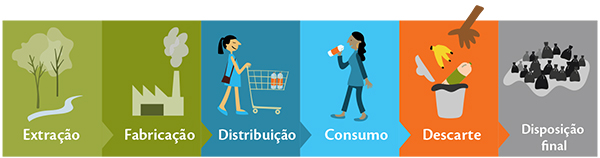
\includegraphics[width=10cm]{images/EconomiaLinear.png}
    \caption{Ilustração da Economia Linear}
    \UrlFont{bulbeenergia.com.br}
    \label{fig:economia_linear}
\end{figure}

Tendo em conta que as matérias-primas são finitas e o crescimento populacional é cada vez mais acelerado, torna-se evidente a necessidade de um novo modelo de produção, que vise o desenvolvimento sustentável invés da produção em massa.

Dessa necessidade, surgiu o conceito da Economia Circular. Tem por base os seguintes pressupostos: "redução, reutilização, recuperação e reciclagem de materiais e energia"\cite{EconomiaCircular}.

\begin{figure}[ht]
    \centering
    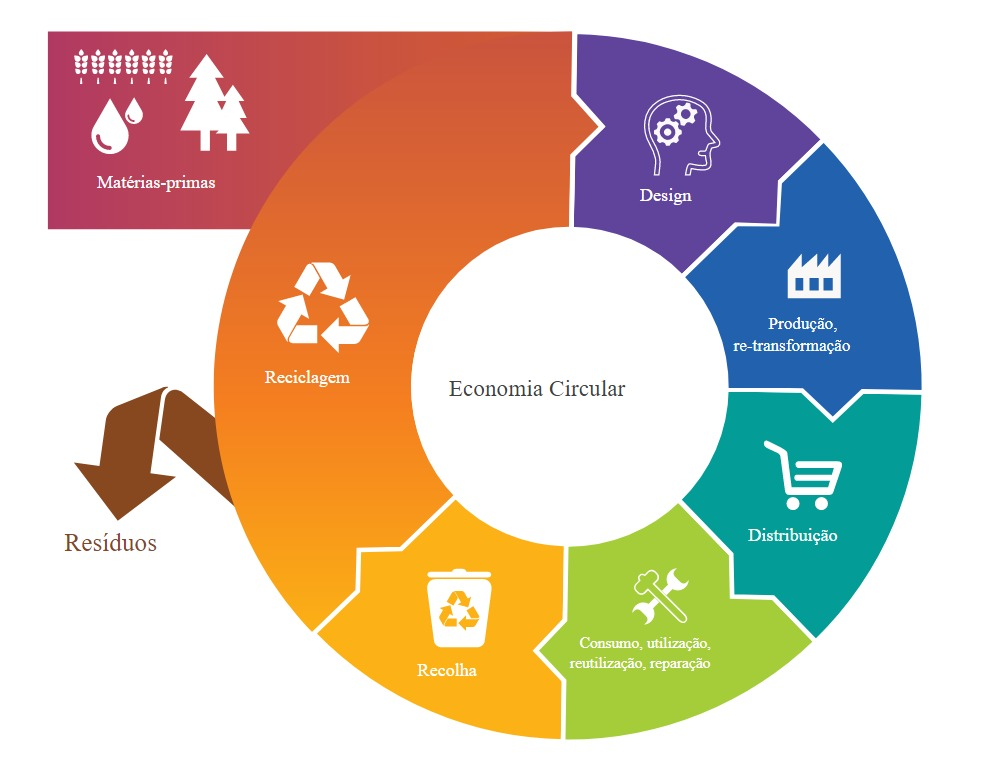
\includegraphics[width=7cm]{images/Economia_Circular.jpeg}
    \caption{Ilustração da Economia Circular}
    \UrlFont{www.europarl.europa.eu}
    \label{fig:economia_circular}
\end{figure}

Como podemos observar na Figura \ref{fig:economia_circular}, a economia circular espelha-se no ciclo dos ecossistemas. Para tal, os componentes técnicos dos produtos são planeados atempadamente com o intuito de serem facilmente reutilizados, renovados e atualizados\cite{EconomiaCircular1}. Graças a este maior planeamento, os produtos passam a ter uma vida útil maior. Por sua vez, faz decrescer a necessidade de uma produção em massa, reduzindo o lixo residual.

\begin{wrapfigure}[15]{l}{7cm}
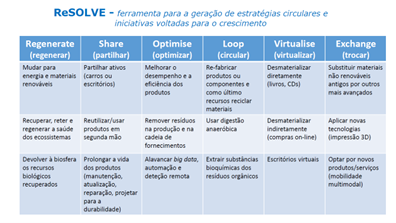
\includegraphics[width=7cm]{images/Resolve.png}
\caption{Tabela representativa das medidas que se enquadram nos pontos essenciais da Framework ReSOLVE.}\label{wrap-fig:1}
\UrlFont{moodle.isep.ipp.pt}
\end{wrapfigure}

Outro pilar fundamental da economia circular é o uso de energias renováveis e o respeito pela biodiversidade. Uma das ferramentas utilizadas para a geração de estratégias circulares e iniciativas voltadas para o crescimento é a \textit{framework ReSOLVE} \cite{EconomiaCircular1}. 

Com o intuito de conhecer melhor a Replai, perguntamos-lhe em quais pontos a empresa enquadra-se nos alicerces da filosofia ReSOLVE, obtivemos a seguinte resposta:\begin{quote}
"A Replai encaixa-se em dois pontos o \textit{Optimise} e o \textit{Virtualize}."\end{quote}

O conceito Optimise, visa a eficiência do produto desenvolvido. O produto desenvolvido pela Replai trata-se de um analisador de vídeos fazendo uso da inteligência artificial. Posto isso, o trabalho de análise anteriormente desenvolvido pelos colaboradores passa a ser da responsabilidade do software desenvolvido com a ajuda da inteligência artificial. Dessa forma, passamos a ter um processo automático e otimizado. 

Outro conceito em que a Replai se encaixa é o Virtualize. Visto que a empresa cria vídeos publicitários de acordo com as tendências do mercado, o processo criativo que antes era da responsabilidade dos colaboradores passa a ser da responsabilidade de um software com suportes tecnológicos. 

Tendo em conta que a empresa em questão desenvolve \textit{Software}, uma boa prática e sugestão seria focar no conceito de \textit{Share}. Esse conceito tem por base um maior ciclo de vida dos produtos desenvolvidos. Para que isso aconteça, a empresa necessita de um planeamento prévio do produto a ser desenvolvido para futuramente ser possível aplicar atualizações ao mesmo, conseguindo, dessa forma, prolongar o seu ciclo de vida e reduzir os gastos envolvidos na produção de um novo.

\section{Planeamento}
\subsection{Níveis de Gestão}
    Grande parte das empresas seguem a hierarquia de gestão apresentada na figura \ref{fig:hierarquia_gestao} e a Replai é uma delas. No entanto reparamos que diverge da regra geral.

    \begin{figure}[h]
        \centering
        \includegraphics[width=7cm]{images/Hierarquia de gestão.png}
        \caption{Níveis na Hierarquia de Gestão}
        \label{fig:hierarquia_gestao}
    \end{figure}

    Esta tem três gestores de topo, dos quais dois são fundadores da empresa. Um está responsável pelas vendas, \textit{Chief Sales Officer} (CSO), e o segundo fundador está responsável pelo produto, \textit{Chief Product Officer} (CPO). Por fim, o último gestor de topo é um \textit{Chief Director of Technology}.

    A empresa acredita que o conceito de gestores intermédios não traz benefícios à organização e dão o exemplo do jogo do telefone estragado, onde a mensagem da primeira pessoa chega ao fim da linha distorcida. Os gestores intermédios seriam mais um nível onde a mensagem iria diluir ou ficar presa. A informação deve fluir livremente entre camadas, e quantas mais houverem, mais resistência irá haver para que essa informação passe entre elas. Devido à dimensão da Replai, não existem recursos humanos nem gestores de \textit{financing}, logo, este trabalho é passado aos gestores de topo, e caso necessário, é efetuada por terceiros.
    
    Há varias equipas nas secção de vendas da Replai e cada equipa tem um diretor que é considerado gestor de primeira linha. Nas vendas, temos os \textit{Business Developers}, onde o seu maior objetivo é trazer fluxo de clientes que estejam interessados em comprar à Replai. Temos \textit{Account Management} que têm como objetivo manter clientes e impedir que estes cancelem o contrato. Existe também \textit{Customer Success}, que são responsáveis por um \textit{onboarding} eficaz dos clientes, ou seja, integrá-los devidamente na empresa, trabalhando lado a lado com os \textit{account managers}.
    
    Saindo das vendas, temos a secção da tecnologia: o \textit{Director of Technology}, que tem como objetivo reduzir ao máximo o número de \textit{bugs} e garantir a boa funcionalidade da plataforma e o \textit{Tech Lead Manager}, que vigia a qualidade do \textit{software} desenvolvido pela equipa.
    Por fim, o \textit{CPO} tem como objetivo manter a visão alinhada do produto e entregar as funcionalidades com mais alto impacto e menos custo. Dentro do produto, temos uma maior variedade de equipas que contêm funcionários não gestores. Por exemplo, o não gestor do \textit{design}, tem como objetivo resolver problemas e fazer o mínimo \textit{design} possível. Diogo afirmou que, tal como o \textit{Software Development}, um bom design é uma coisa que se deve que fazer pouco \textit{design}, ou seja, resolver os problemas com o mínimo de impacto possível. Os engenheiros têm como objetivo desenvolver requisitos de maneira a que se mantenham o mais sustentável possível e devem implementá-los com qualidade. Existe uma equipa de pesquisa que tem um \textit{Research Lead}, cujo objetivo é trazer informação que seja centrada no utilizador, ou seja, descobrir o que o utilizador realmente quer e é considerado a única área da empresa que não é influenciada.
    
    
\newpage
\subsection{Políticas de Planeamento}
    Sendo a Replai uma empresa voltada para área das tecnologias informáticas, a empresa organiza-se por equipas, que por sua vez adotam metodologias e tecnologias divergentes para organizar o seu trabalho. Um ponto em comum entre todas as equipas é a existência de um responsável por cada área de atuação da empresa. 
    
    \begin{wrapfigure}[16]{r}{6cm}
        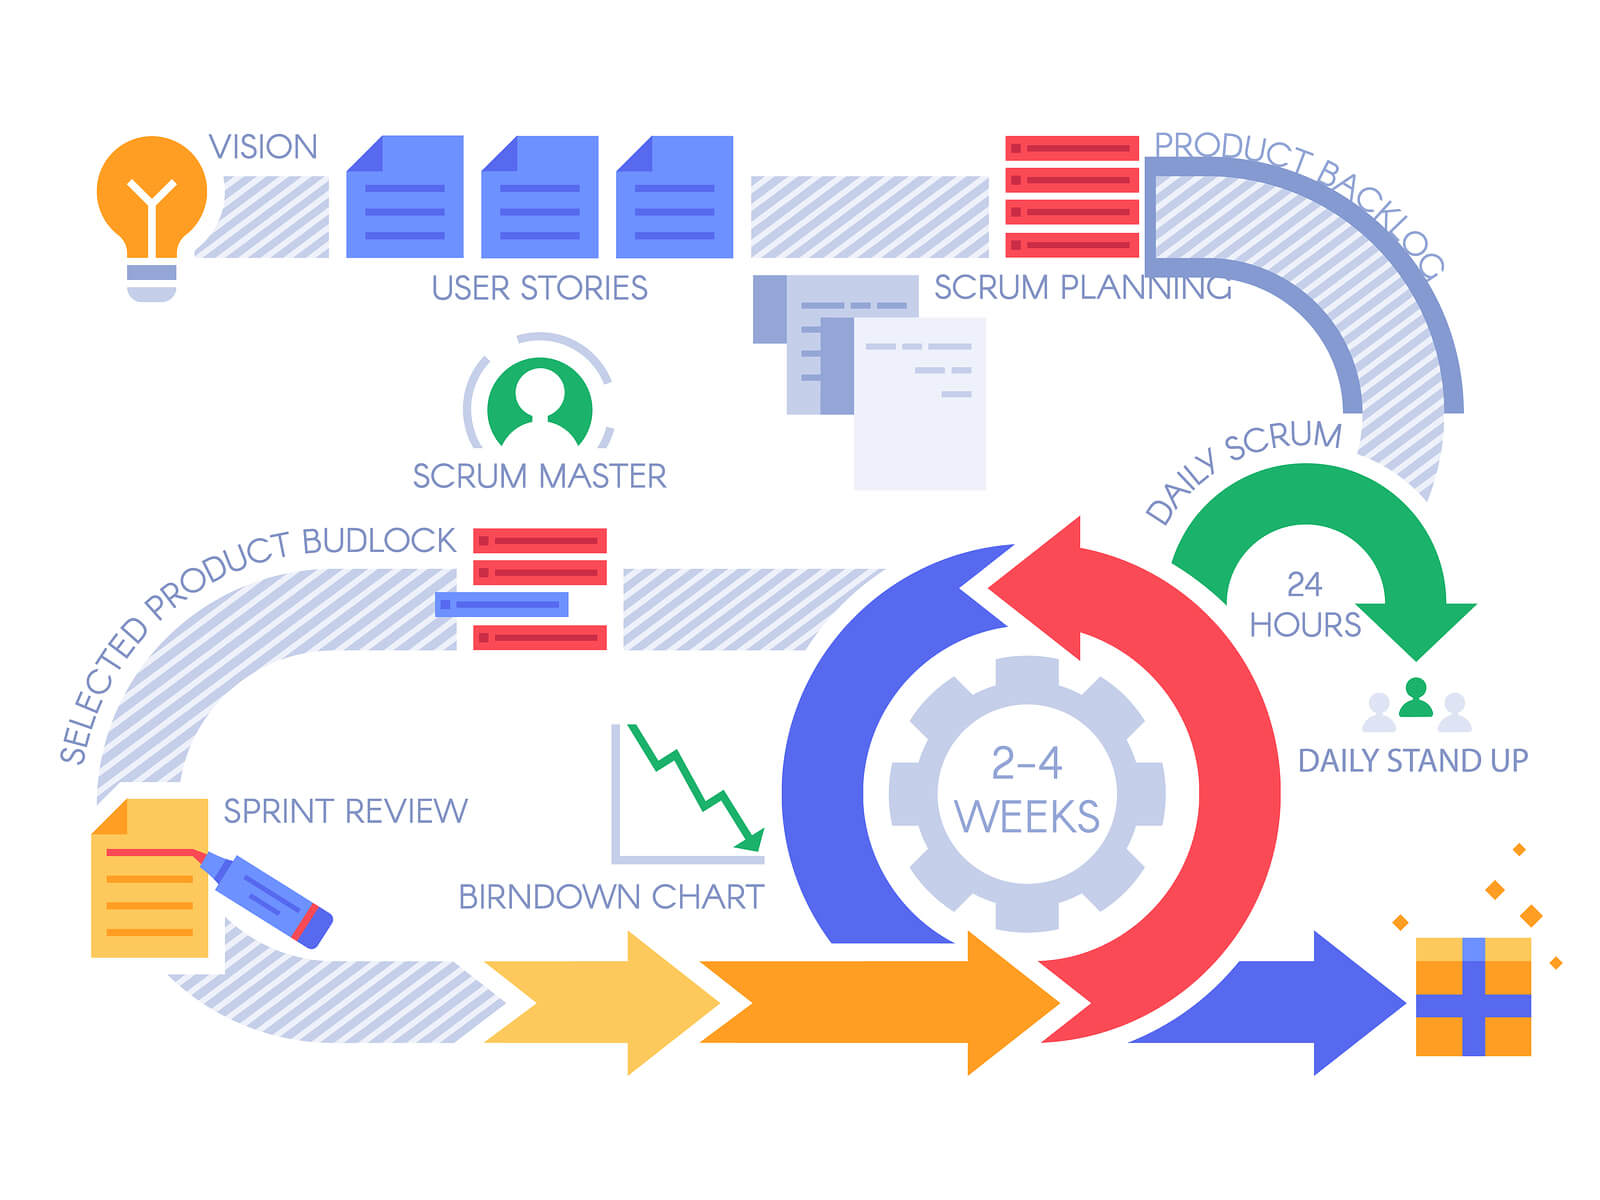
\includegraphics[width=5.5cm]{images/Innovación-ágil.png}
        \caption{Representação da metodologia Scrum.}\label{wrap-fig:2}
        \UrlFont{digite.com}
    \end{wrapfigure}
    
    A metodologia ágil adotada pela empresa é a Scrum. Caracteriza-se essencialmente pela divisão do trabalho em \textit{sprints}, realização de breves reuniões diárias e revisão do trabalho desenvolvido no término de cada \textit{sprint}. 
    
    Na Replai, os \textit{sprints} tem a duração de duas semanas. A distribuição de tarefas é feita usando os casos de uso do sistema, porém, os funcionários também podem exercer tarefas de investigação. Caso os colaboradores possuam tarefas de investigação recebem uma menor quantidade de casos de uso, para que não haja sobrecarga.
    
    Depois de feita a distribuição das tarefas, cada equipa faz uso de ferramentas específicas para gerenciar o seu trabalho. Por exemplo, a equipe de venda faz uso do \textit{software} HubSpot para organizar o plano de vendas da empresa e manter o registo dos potenciais clientes. Já a equipe de desenvolvimento faz uso da ferramenta Jira, que permite gerir a distribuição dos casos de uso entre os colaboradores e no final de cada \textit{sprint} gerar gráficos que são pertinentes para analisar e debater o trabalho desenvolvido até o momento e refletir sobre as boas ou más práticas que devem ser mantidas ou alteradas para o próximo \textit{sprint}.  
    
    No final do desenvolvimento de cada projeto é feito um gráfico da velocidade de produção. Esse gráfico é a razão entre o número de casos de uso finalizados em todos os \textit{sprints} sob a número de \textit{sprints}. A partir desse resultado é possível planear/ajustar os projetos com base na média de trabalho das equipas.

\subsection{Planeamento Organizacional}

As equipas de trabalho, para desenvolvimento de software, recorrem à metodologia Agile Scrum. As user stories são definidas como objetivos claros e mensuráveis, de forma a permitir alcançar as metas definidas, story points.
  
Contudo, para tarefas que podem requerer, por exemplo, investigação, recorrem a time boxes, que permitem alocar uma quantidade fixa e máxima de recursos que poderão ser dedicados a uma dada tarefa.
  
Como dito pelo Diogo na entrevista, se uma determinada tarefa não for de fácil análise e não for possível mensurar a mesma, esta irá prejudicar o fluxo da equipa e, também, demonstrará que a divisão do trabalho necessário não foi efetuada corretamente.


\subsection{Valores, Visão e Missão da Replai}

Como mencionado na caracterização, o serviço prestado pela Replai é diferente da visão inicial, visto que o mesmo possuía certas falhas.

Apesar de a visão da empresa ter sido ligeiramente alterada, a sua missão e o seu plano estratégico (transição governamental para empresarial) baseia-se na mesma ideia: perceber como um vídeo funciona! Desta forma a visão da Replai é ser um fator essencial nas empresas do mundo \textit{gaming} criarem a cultura mais enriquecida no mundo dos \textit{esports}. A missão da Replai é ajudar as empresas a aumentar a adesão, lealdade, e entusiasmo dos amantes de \textit{gaming} perante a sua marca \textit{esports}.

A empresa descreve-se como sendo desafiante, destemida, dedicados ao desenvolvimento do melhor produto e extremamente abertos a ideias novas, sugestões e uma comunidade saudável para poderem ter um excelente ambiente de trabalho!

\subsection{Cadeia de Valor}
A cadeia de valor caracteriza-se como sendo o processo de agregar valor as atividades desenvolvidas pela empresa, seja ela a confeção de novos produtos ou serviços. 

\ Esse processo tem como principal função ajudar as empresas a compreenderem o seu funcionamento e por consequência, melhorar o seu processo produtivo.
Para compreendermos melhor como a cadeia de valor funciona, Michael Porter criou uma divisão teórica que nos ajuda a compreender esse processo. Para tal, subdividiu o processo em dois tipos de atividades: primárias e de suporte\cite{CadeiaDeValor1}.

\ As atividades primárias também chamadas de processos \textit{Core}, são todas aquelas que geram benefícios diretos para os clientes. Essas atividades são as seguintes:\\

\textbf{-Logística de entrada:}  Refere-se ao relacionamento com fornecedores, aquisição de matéria-prima e contratações de serviços.\\

\textbf{-Operações:} Refere-se ao processo de criação de um produto ou serviço.\\

\textbf{-Logística de saída:} Refere-se as atividades de entrega do produto/serviço ao consumidor final.\\

\textbf{-Marketing e vendas:} Refere-se aos processos utilizados para atrair consumidores. \\

\textbf{-Serviços:} Refere-se as atividades de suporte ao produto/serviço.\\

\ Tendo por base esses conceitos, iremos analisar as atividades primárias realizadas pela Replai. 

\ Em relação a Logística de entrada, sendo a empresa voltada para a área de informática, a “matéria-prima” utilizada para a criação dos seus produtos são novas ideias e pesquisas. 

\ Referente as Operações, a Replai divide a criação de um produto/serviço em 4 etapas: Análise, Pré-Planeamento, Refinamento e Planeamento e Execução. Cada uma dessas fases é caracterizada por inputs e outputs expectáveis, como representado na figura abaixo.
    \begin{figure}[ht]
       \centering
        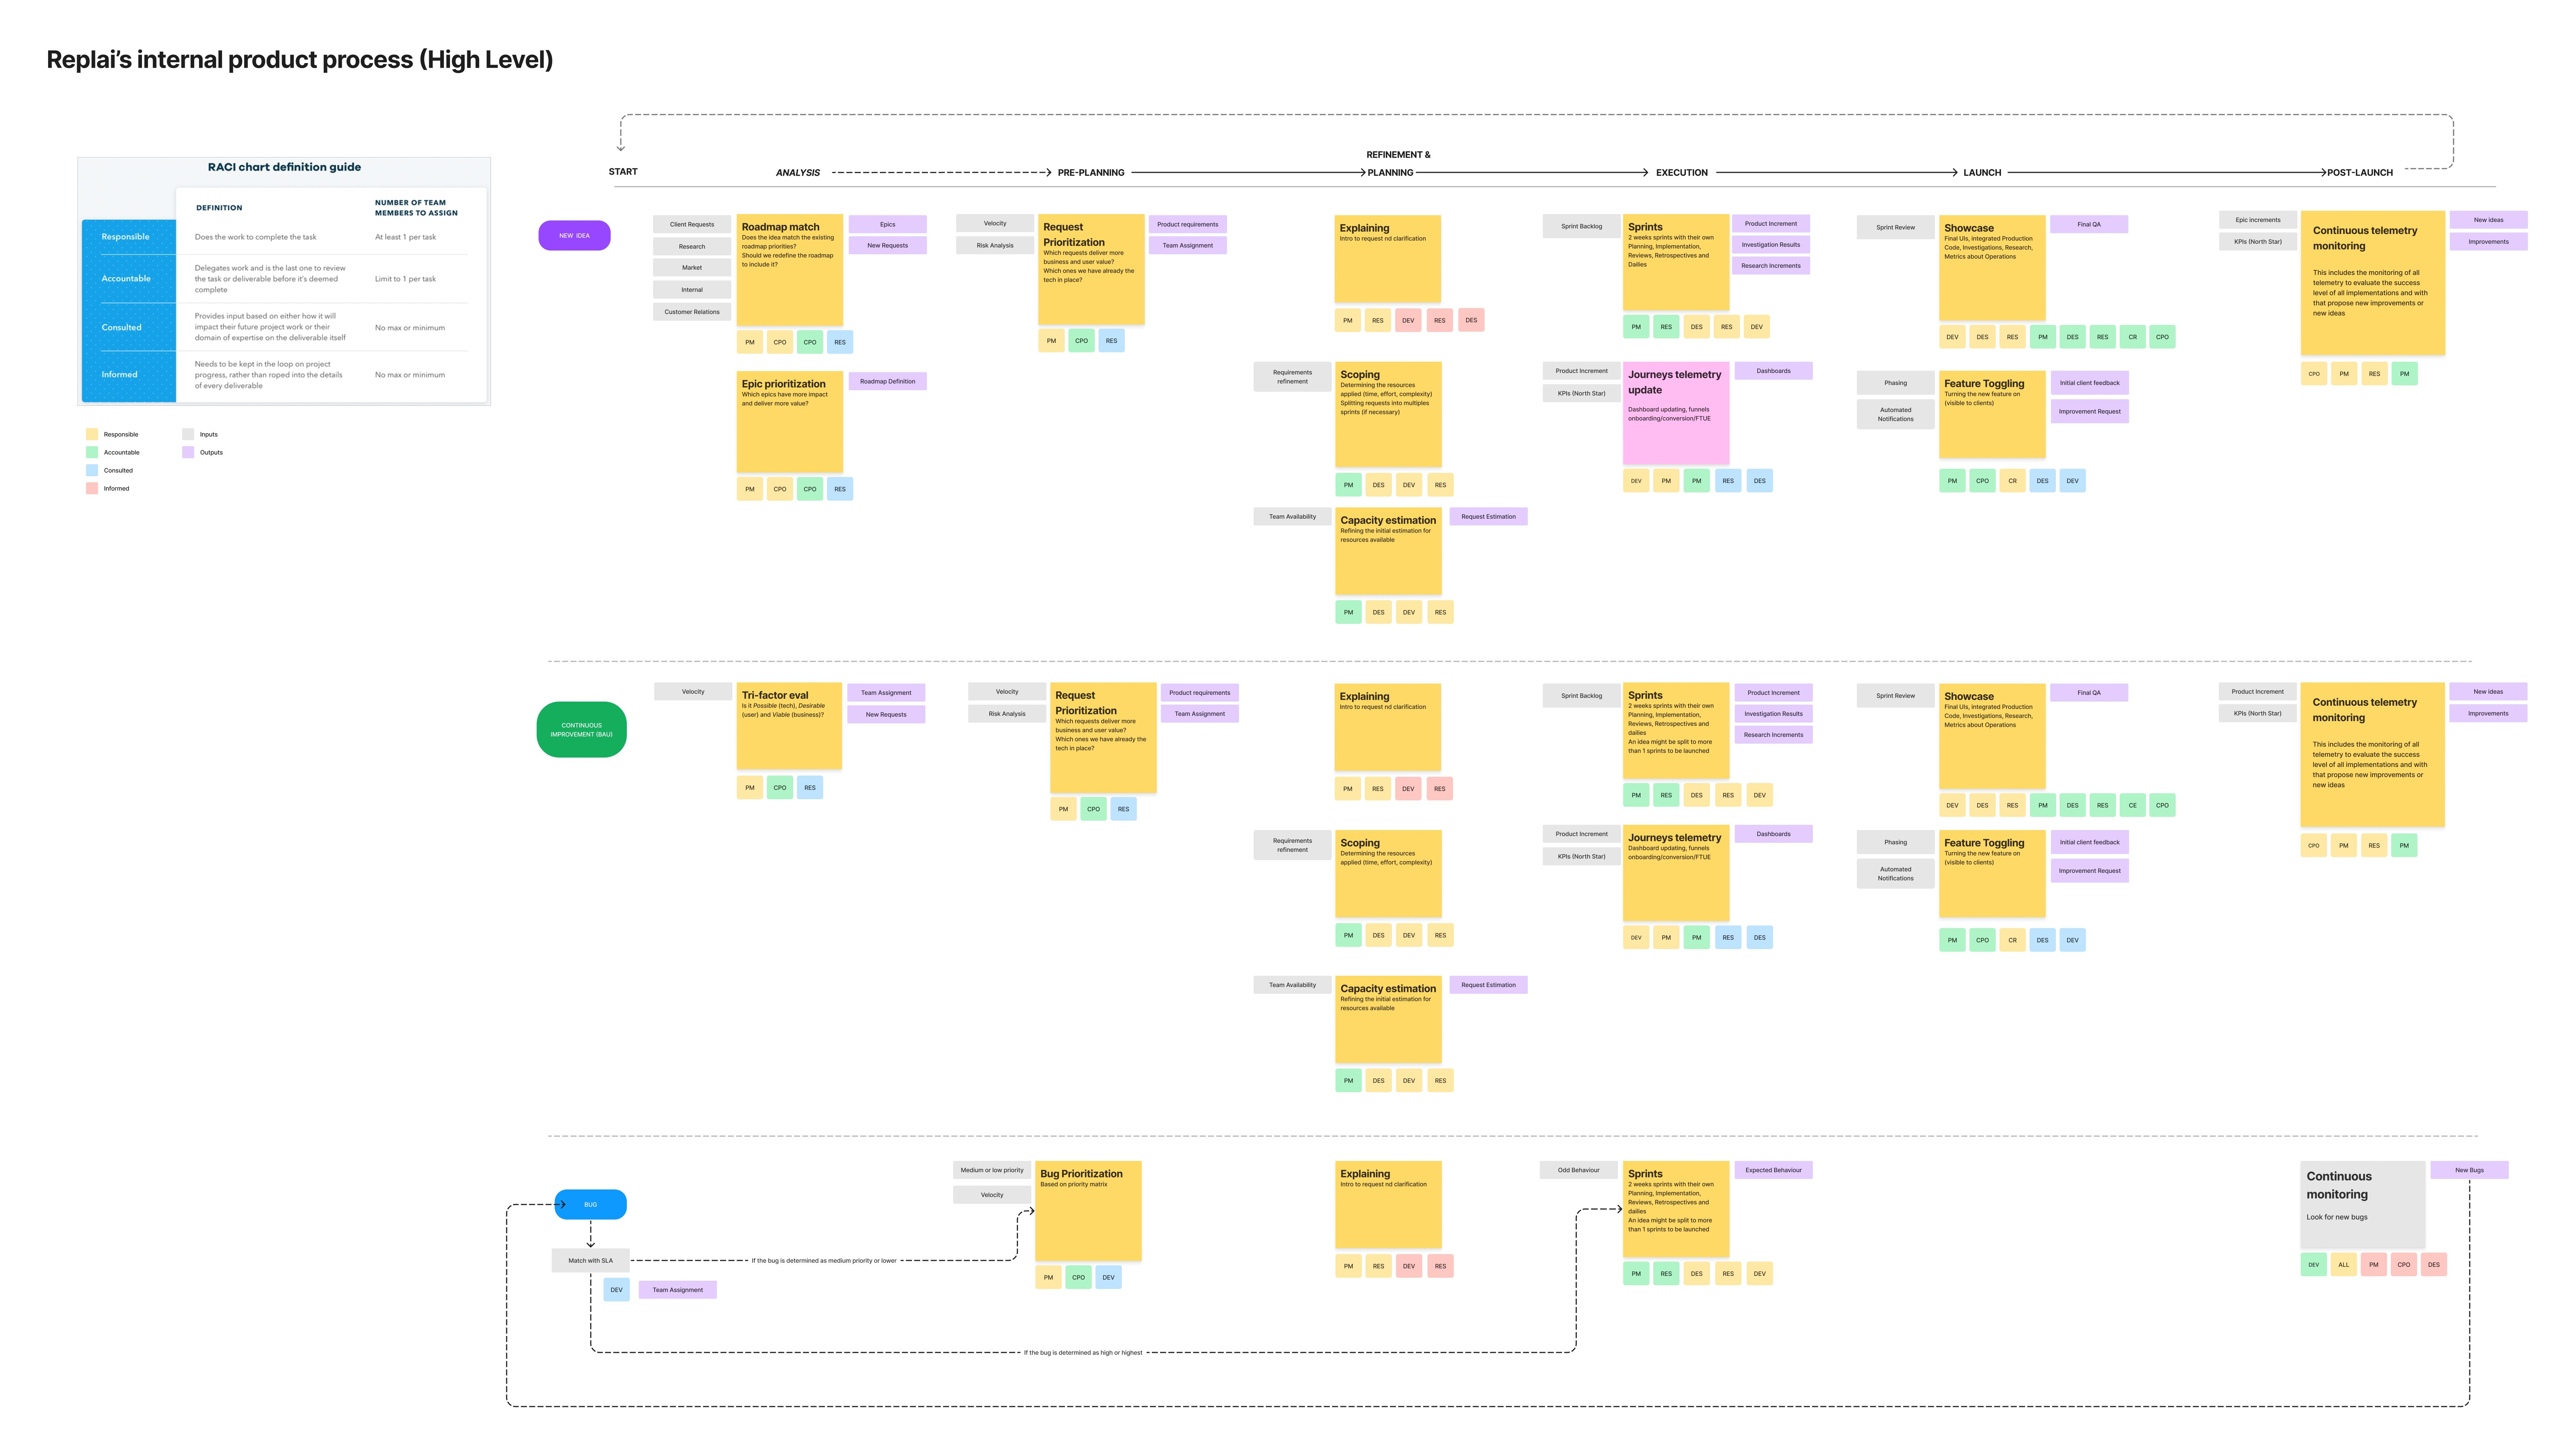
\includegraphics[width=11cm]{images/Replai-Process.jpg}
        \caption{Etapas de desenvolvimento de um projeto na Replai.}
        \label{fig:replai_processo}
    \end{figure}\\

\ Passando ao ponto referente a Logística de saída esse é feita de forma totalmente virtual visto que e empresa desenvolve Software.

\ Relativamente as estratégias de Marketing utilizadas pela empresa, as principais são: a divulgação de novos produtos pelas redes sociais e a estratégia de libertar novas funcionalidades em fases e com públicos alvos específicos, para conseguir captar a atenção e despertar interesse continuo pelo produto.

\ Por último temos os Serviços, na Replai existe uma equipa de suporte para atender a eventuais problemas relacionados com o produto adquirido pelos seus clientes.\\

\ Já as atividades de suporte caracterizam-se por gerarem valor indiretamente para empresa pois, dão suporte as atividades primárias\cite{CadeiaDeValor}.Essas atividades são as seguintes:\\

\textbf{-Infraestrutura:} Refere-se a gestão administrativa, legal e financeira\cite{CadeiaDeValor} da empresa.\\

\textbf{-Gestão de Recursos Humanos:} Refere-se ao processo de aquisição de novos colaboradores e capacitação dos já existentes.\\

\textbf{-Desenvolvimento Tecnológico:} Refere-se a automatização dos processos da empresa. \\

\textbf{-Aquisição/compras:} Refere-se essencialmente a negociação com os fornecedores e busca de matérias-primas.\\

\ Tendo por base esses conceitos, iremos analisar as atividades de apoio realizadas pela Replai.

\ Em relação a Infraestrutura, a gestão legal e financeira é feita através de serviços terceirizados.

\ Quanto aos recursos humanos, atualmente está a cargo do fundador da Replai, sendo este o responsável pela contratação de novos colaboradores assim como oferecer formação continua aos seus empregados atuais.

\ Relativamente a automatização de processos, a Replai possui uma política de contratação de \textit{freelancers} para desenvolverem tarefas genéricas que não envolvam o contexto de domínio de negócio do projeto que está a ser desenvolvido. Dessa forma, otimizam o seu trabalho, podendo aplicar o seu tempo em tarefas mais complexas.

\ Passando ao último ponto, A aquisição/compra, sendo a Replai uma empresa voltada ao desenvolvimento de \textit{software}, não existe grande relação com fornecedores e compra de matéria-prima. 





\subsection{Análise do ambiente competitivo}
\begin{quote}
    "Uma organização é sempre inseparável do espaço em que se coloca"\cite{Planeamento}
\end{quote} e portanto, é importante fazer uma análise dos fatores externos e internos nos quais podem por em causa o sucesso da empresa. A investigação e análise constante destas características  é o que possibilita as empresas permanecerem competitivas na sua longevidade. A este conjunto de fatores no ambiente externo com os fatores do ambiente interno denomina-se ambiente competitivo.

Para uma melhor compreensão dos ambientes que coexistem no espaço da empresa, identificasse três tipos de ambientes: \\

	\textbf{-Ambiente externo geral:} Neste ambiente são analisados fatores que estão fora do controlo direto da empresa. Estes elementos são características que todas as organizações do mundo enfrentam, independentemente do seu setor de atividade. \\
	

	\textbf{-Ambiente externo especifico:} O ambiente externo específico avalia o grau de competitividade do setor que uma organização está ou se pretende colocar.  Neste ambiente qualifica-se o grau de atratividade assim como se analisa indicadores de entrada ou saída do mercado.\\

	\textbf{-Ambiente interno:} Em suma, o ambiente interno é o responsável pela análise do sucesso e funcionamento da organização, isto é, que vantagens competitivas e fraquezas a organização apresenta para o mercado do setor de atividade em que se encontram. \\
	
	
\newpage
\subsubsection{Análise PEST}
Para análise do ambiente externo geral recorre-se a uma ferramenta denominada Análise PEST. Sendo PEST um acrónimo resultante do acoplamento das iniciais: Políticos (P), Económicos (E), Sociais(S), Tecnológicos (T). \\

%Dito isto,"PEST" refere-se respetivamente a: \\


\noindent \textbf{Fatores políticos} %, fatores que incluem questões legais e regulamentares como por exemplo, Política Fiscal e Regulações Ambientais.
\begin{itemize}
    \item A Replai, sendo uma empresa sem sede, no entanto, multinacional, está dependentes das políticas fiscais relacionadas com empresas digitais e e-commerce.
    \item Como a empresa tem clientes por todo mundo, é necessária uma elevada atenção à legislação e estabilidade governamental dos países colaboradores.
\end{itemize}

\underline{Exemplos Práticos}:
\begin{itemize}
    \item Devido à guerra, e sendo que a Replai tem colaboradores ucranianos, alguns clientes viram-se forçados a desistir e deixar de usufruir dos produtos da empresa.
    \item Consequentemente os conflitos políticos dificulta a adesão de clientes russos e/ou ucranianos \\
\end{itemize}


\noindent \textbf{Fatores Económicos} %, estes abordam o poder de compra da organização e o custo capital, para analisar temos que verificar que efeitos, por exemplo, de que forma as taxas de câmbio, inflação  juros afetam a empresa.
\begin{itemize}
    \item Como a Replai se sustenta através de rondas de investimentos, esta está  sujeita ás condições presentes na legislação relativa a investimentos.
    \item Altamente suscetíveis à inflação e ao valor que os investidores atribuem à Replai.
\end{itemize}

\underline{Exemplos Práticos}:
\begin{itemize}
    \item A Replai sustenta-se através de rondas de investimento. Devido à recessão atual derivado da pandemia e da guerra, uma das rondas de investimento não foi concretizada apesar dos resultados obtidos pela empresa, isto resultou numa mudança de estratégia de sustento da empresa de \textit{hypergrowth}, para cobrir despesas primeiro e assegurar lucros.\\
\end{itemize}


\noindent \textbf{Fatores Sociais} %, que incluem fatores culturais e distribuições geográficas da organização, inclui exemplos como estilos de vida, hábitos consumo e distribuição etária. \\
\begin{itemize}
    \item A faixa etária consumidora de vídeos tem alargado, um ponto fulcral para a Replai pois origina mais possíveis clientes.
    \item Está presente na era digital, onde o consumo de vídeos é abundante.\\
\end{itemize}

\noindent \textbf{Fatores Tecnológicos} %, o fator que aborda a terceirização da empresa. Avaliada através dos processos de investigação e automação da empresa. \\
\begin{itemize}
    \item A possibilidade de inovação tecnológica neste ramo é alta, pois é um mercado pouco saturado.
    \item A possibilidade de evolução tecnológica em produtos já existentes é igualmente elevada, já que há muita procura e pouca oferta. 
\end{itemize}

\underline{Exemplos Práticos}:
\begin{itemize}
    \item Tiktok, a plataforma de partilha e criação de vídeos curtos, lançou recentemente um algoritmo avançado de estudo de tendências e métricas relevantes para o sucesso de publicidades. Isto inicialmente apresentou-se como uma ameaça, no entanto, como a Replai se especializa no mercado gaming, acabou por não ser afetada totalmente.
\end{itemize}
\newpage
\subsubsection{Análise de Porter}
Questionamos o Diogo, \textit{Project Manager}, relativamente ao modelo das cinco forças de Porter, como mostra a figura \ref{fig:Porter}, e como ele avalia essas forças no impacto da rendibilidade da organização.

\begin{figure}[ht]
    \centering
        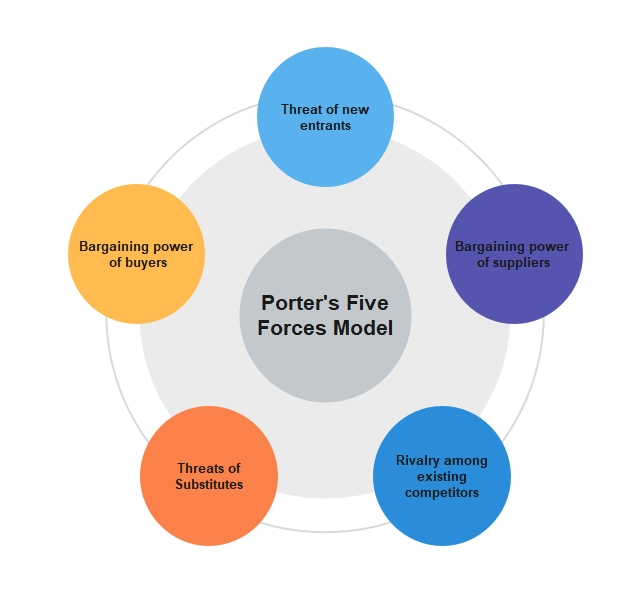
\includegraphics[width=10cm]{images/porters-five-forces-model.jpg}
        \caption{Cinco forças de Porter}
        \label{fig:Porter}
\end{figure}

\noindent\textbf{Rivalidade entre os concorrentes existentes:}\\

O espaço onde a Replai se encontra ainda está muito inexplorado, logo todas as empresas, que são poucas, estão à caça do \textit{market share}. Todas as abordagens entre os concorrentes são muito parecidas. Apesar do Diogo ser influenciado, afirma que a Replai tem uma abordagem muito diferenciadora da concorrência, à parte de uma outra empresa. Esta é a que tem mais sucesso nesta competição, está muito avançada, mas é vista pelo Diogo como sendo uma parte adjacente a todo o processo e não um concorrente direto. 

Concluímos com o Diogo que o facto de serem poucas empresas é uma força \underline{Fraca}, e também tivemos em conta que todas as empresas estão à procura do maior market share possível, o que consideramos ser uma \underline{Grande} força. Logo a força que o Diogo usou para caracterizar a rivalidade entre os concorrentes existentes foi \textbf{\underline{Moderada}}.\\

\noindent\textbf{Poder negocial dos fornecedores:}\\

A Replai sendo uma empresa de software, de momento tem o único fornecedor, a Amazon. Como esta empresa, há muitas que oferecem os mesmos serviços. Mudar de fornecedor também é extremamente fácil e sem qualquer custo para a empresa a não ser o custo de serviço.

Sendo assim, chegamos a uma rápida conclusão com o Diogo. Haverem muitas empresas a fornecerem o mesmo serviço é, para a Replai, uma força \underline{Fraca}, e a facilidade de como podem alterar de fornecedor é também uma força \underline{Fraca}, sendo então o Poder negocial dos fornecedores, uma força \textbf{\underline{Fraca}}.\\

\newpage
\noindent\textbf{Ameaça de novos concorrentes:}\\

Foi-nos falado de um momento importante na história que marcou o mercado da Replai. A Apple removeu um identificador dos iPhones com o iOS14, identificador que dava o perfil do utilizador, no que conta a publicidade. Sendo este removido, muitas empresas que queriam conhecer os seus clientes para lhes fornecer publicidades ficaram sem forma de o fazer, criando assim, uma grande procura em empresas como a Replai. Cada vez mais surgem novas empresas a tentar fazer exatamente o mesmo que ela faz. O Diogo contou-nos que já há algum feedback do que corre mal e do que corre bem, mas que não há solução perfeita. Solução esta que de acordo com ele não existe, deu como exemplo a Google, que não é uma solução perfeita, mas é uma solução ótima. 

Neste mercado da Replai ainda não existe uma solução ótima, e há sempre uma chance moderada de um novo concorrente encontrar essa solução, Diogo classifica este facto como sendo uma força \underline{Forte}. Como este mercado está a ter cada vez mais procura, o Diogo vê o aparecimento de muitas novas empresas como uma força \underline{Forte}. Concluindo assim que a ameaça de novos concorrentes é uma força \textbf{\underline{Forte}}.\\

\noindent\textbf{Poder negocial dos clientes:}\\

O mercado da Replai é maioritariamente \textit{Business to Business}, logo os clientes são entidades, o que significa que há um numero baixo de clientes, sendo eles todos muitos importantes para a empresa. O Diogo deu-nos exemplos de grandes empresas que são seus clientes como a Activision, a Zinga, Rovio, entre muitos outros, e perder esse clientes vinha com um grande custo para a Replai.

Tendo isto tudo em conta, depreendemos que ao haver muitos poucos clientes, estes tem uma \underline{Grande} força no poder negocial. Da forma que o mercado da Replai funciona, todos os clientes são grandes empresas, o que faz delas clientes muito importantes, fazendo com que estes tenham também uma \underline{Forte} força. Em suma o poder negocial dos clientes é caracterizado como sendo, uma força \textbf{\underline{Forte}}.\\

\noindent\textbf{Ameaça de produtos substitutos:}\\

O Diogo diz que a Replai é das empresas mais caras, senão a mais cara. Apesar dos seus cliente serem maioritariamente grandes organizações, ou indivíduos com grande poder de compra, existe sempre a preocupação dos clientes tenderem para produtos mais baratos. Para contrariar esta preocupação, sabe-se que nenhum outro produto é considerado a solução ótima, como já foi previamente referido, então não há garantias de que os esses produtos possa substituir o que a Replai tenha para oferecer. O Diogo confirma também que esta é muito diferenciadora em comparação com a competição.

Concluímos assim que há uma \underline{Grande} força que afeta a Replai por eles serem dos produtos mais caros no mercado, por outro lado, não se pode dizer que as outras empresas a possam substituir, logo o Diogo considera que este aspeto tenha uma \underline{Fraca} força. Fazendo, por fim, com que a ameaça de produtos substitutos seja uma força \textbf{\underline{Moderada}} para a Replai.\\

\newpage
\subsubsection{Análise VRIO}

O modelo VRIO (Valor, Raridade, Imitabilidade e Organização, respetivamente) permite avaliar \textit{assets} de uma determinada empresa, ao sujeitarmos a qualidade em questão a estes 4 parâmetros.
  
Iremos usar o seu algoritmo e a capacidade de organização e adaptabilidade como recurso e competência, respetivamente, no estudo através desta \textit{framework}.\\

\begin{figure}[ht]
    \centering
        
\includegraphics[width=7cm]{images/vrio.png}
        \caption{Framework VRIO}
        \label{fig:vrio}
\end{figure}

\noindent \textbf{Recurso:} \\

\noindent \textbf{Valor}\\
 
O algoritmo por trás do produto da Replai é, possivelmente o seu recurso mais forte. Através do  mesmo, a empresa consegue vender as métricas e os marcadores que representam a análise dos conteúdos dos consumidores.
  
Numa sociedade em que quotidianamente, a expansão do consumo de vídeo dá-se exponencialmente, seja para empresas ou criadores de conteúdo, o sucesso do vídeo, por exemplo, a nível publicitário, é um fator para a expansão de uma determinada organização.\\

\noindent \textbf{Raridade e Imitabilidade}\\

Dado que foi desenvolvido pioneiramente e permanece com um resultado único no mercado, o mesmo é também raro e imitável, visto que se encontra patenteado. Existem produtos com princípios de funcionamento semelhantes, contudo, com uma visão de análise distinta da Replai.\\

\noindent \textbf{Organização}\\
  
Aproveitando o seu recurso exclusivo, a empresa facilita o acesso ao mesmo por parte do utilizador. Faz isso através de interfaces simples, interpretação em temo real e uma integração profunda do seu produto com as maiores plataformas de vídeo, como o Youtube.
  
A remoção do atrito entre a disposição de resultados e a interpretação dos utilizadores por meio de diagramas e painéis de utilizador permitem uma experiência autónoma e intuitiva.\\

\noindent \textbf{Competência:}\\

\noindent \textbf{Valor}\\

Desde a sua fundação que tinha como visão serem uma empresa \textit{user centered} e com um workflow estruturado, algo essencial em ambiente de \textit{start-up}, dado que os recursos são limitados. Não só isso, mas equipas devidamente geridas e com objetivos claros e atingíveis, são propensas a uma produtividade e motivação superior, beneficiando o projeto em que trabalham.\\

\noindent \textbf{Raridade e Imitabilidade}\\
  
Como descrito pelo PMO, Diogo Bastos, engenheiros com experiência prévia em grandes centros tecnológicos, tais como \textit{Silicon Valley}, ficaram admirados com a capacidade da Replai.

Considera-se um recurso raro, dado que grandes empresas fazem uso do dinheiro de forma a resolver os problema sem solução para o causador.\\

\noindent \textbf{Organização}\\

Apesar de raro, é possivelmente imitável, contudo, apenas através de boa gestão. Assim, demonstra-se a capacidade organização desta pequena empresa, que impulsiona os “tubarões” da indústria tecnológica (e não só)! 
 

\subsubsection{Análise SWOT}
Com base no que aprendemos até agora, realizamos em conjunto uma análise SWOT da Replai na figura \ref{fig:swot}.\\
\begin{figure}[ht]
    \hspace*{-2.5cm}   
    \centering
    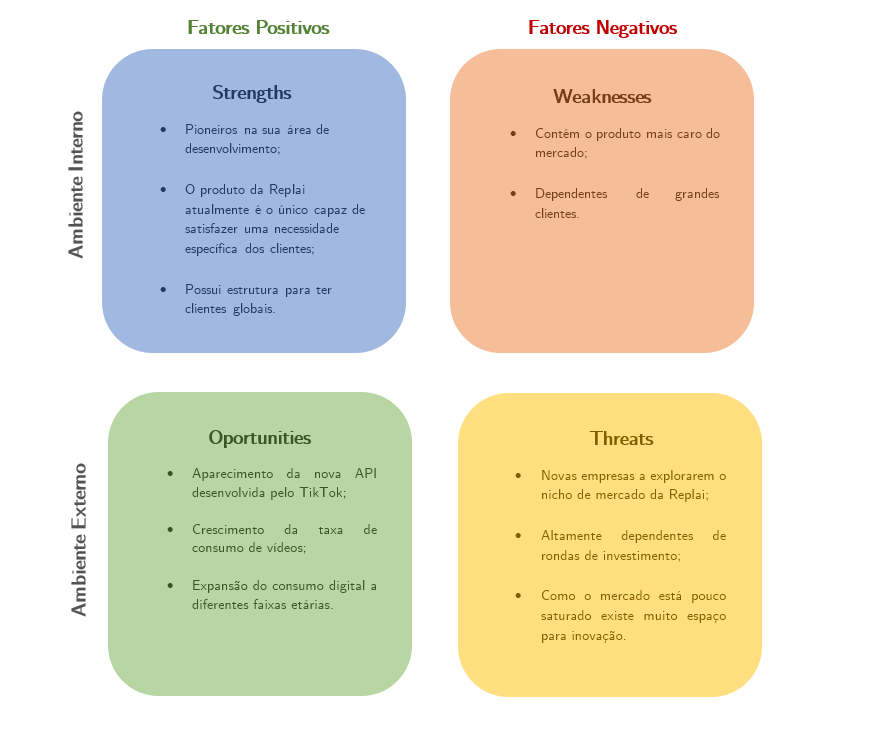
\includegraphics[scale=0.8]{images/SWOT.png}
    \caption{Análise SWOT}
    \label{fig:swot}
\end{figure}

\newpage
\subsection{Possível Estratégia da Organização}
Segundo o processo de planeamento estratégico apresentado na figura \ref{fig:planeamento}, o único ponto que sugerimos uma melhor abordagem é na formulação de objetivos. Apesar da Replai ter objetivos definidos, estes objetivos não estão de acordo com a ferramenta SMART, principalmente no \textit{\textbf{T}}, o ponto temporal. Todos os objetivos são específicos, mensuráveis, atingíveis, e relevantes, nenhum deles nos foi apresentado com uma data de alcance.

\begin{figure}[ht]
    \centering
    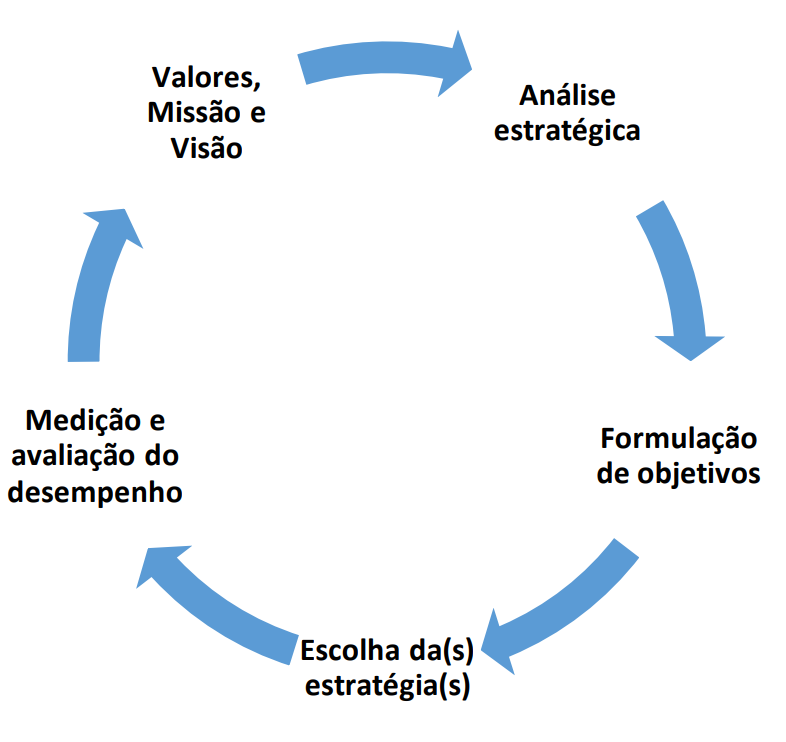
\includegraphics[scale=0.5]{images/planeamento.png}
    \caption{O processo de planeamento estratégico}
    \label{fig:planeamento}
\end{figure}


Perante a análise estratégica, e adaptando ligeiramente os valores, a missão, e a visão da Replai, propomos a seguinte estratégia. Expandir para um novo mercado, possivelmente cinema, já que este tem um publico maior e tem surgido uma interligação entre estes dois setores, para deixarem de estar dependentes de grandes clientes num mercado ainda restringido.

%The \hyperlink{glossary}{\Gls{latex}} typesetting markup language is specially suitable 
%for documents that include \hyperlink{glossary}{\gls{maths}}.

%\newpage    
%\section{Organização}

%\section{Controlo e Sistemas de informação}

%\section{Gestão de Pessoas e Direção}

%\section{Gestão Financeira}

%\section{Marketing}

%\section{Gestão das Operações e Indústria 4.0}







